\documentclass{report}

\documentclass[12pt]{article}
\usepackage{array}
\usepackage{color}
\usepackage{amsthm}
\usepackage{eufrak}
\usepackage{lipsum}
\usepackage{pifont}
\usepackage{yfonts}
\usepackage{amsmath}
\usepackage{amssymb}
\usepackage{ccfonts}
\usepackage{comment} \usepackage{amsfonts}
\usepackage{fancyhdr}
\usepackage{graphicx}
\usepackage{listings}
\usepackage{mathrsfs}
\usepackage{setspace}
\usepackage{textcomp}
\usepackage{blindtext}
\usepackage{enumerate}
\usepackage{microtype}
\usepackage{xfakebold}
\usepackage{kantlipsum}
%\usepackage{draftwatermark}
\usepackage[spanish]{babel}
\usepackage[margin=1.5cm, top=2cm, bottom=2cm]{geometry}
\usepackage[framemethod=tikz]{mdframed}
\usepackage[colorlinks=true,citecolor=blue,linkcolor=red,urlcolor=magenta]{hyperref}

%//////////////////////////////////////////////////////
% Watermark configuration
%//////////////////////////////////////////////////////
%\SetWatermarkScale{4}
%\SetWatermarkColor{black}
%\SetWatermarkLightness{0.95}
%\SetWatermarkText{\texttt{Watermark}}

%//////////////////////////////////////////////////////
% Frame configuration
%//////////////////////////////////////////////////////
\newmdenv[tikzsetting={draw=gray,fill=white,fill opacity=0},backgroundcolor=none]{Frame}

%//////////////////////////////////////////////////////
% Font style configuration
%//////////////////////////////////////////////////////
\renewcommand{\familydefault}{\ttdefault}
\renewcommand{\rmdefault}{tt}

%//////////////////////////////////////////////////////
% Bold configuration
%//////////////////////////////////////////////////////
\newcommand{\fbseries}{\unskip\setBold\aftergroup\unsetBold\aftergroup\ignorespaces}
\makeatletter
\newcommand{\setBoldness}[1]{\def\fake@bold{#1}}
\makeatother

%//////////////////////////////////////////////////////
% Default font configuration
%//////////////////////////////////////////////////////
\DeclareFontFamily{\encodingdefault}{\ttdefault}{%
  \hyphenchar\font=\defaulthyphenchar
  \fontdimen2\font=0.33333em
  \fontdimen3\font=0.16667em
  \fontdimen4\font=0.11111em
  \fontdimen7\font=0.11111em}


%From M275 "Topology" at SJSU
\newcommand{\id}{\mathrm{id}}
\newcommand{\taking}[1]{\xrightarrow{#1}}
\newcommand{\inv}{^{-1}}

%From M170 "Introduction to Graph Theory" at SJSU
\DeclareMathOperator{\diam}{diam}
\DeclareMathOperator{\ord}{ord}
\newcommand{\defeq}{\overset{\mathrm{def}}{=}}

%From the USAMO .tex files
\newcommand{\ts}{\textsuperscript}
\newcommand{\dg}{^\circ}
\newcommand{\ii}{\item}

% % From Math 55 and Math 145 at Harvard
% \newenvironment{subproof}[1][Proof]{%
% \begin{proof}[#1] \renewcommand{\qedsymbol}{$\blacksquare$}}%
% {\end{proof}}

\newcommand{\liff}{\leftrightarrow}
\newcommand{\lthen}{\rightarrow}
\newcommand{\opname}{\operatorname}
\newcommand{\surjto}{\twoheadrightarrow}
\newcommand{\injto}{\hookrightarrow}
\newcommand{\On}{\mathrm{On}} % ordinals
\DeclareMathOperator{\img}{im} % Image
\DeclareMathOperator{\Img}{Im} % Image
\DeclareMathOperator{\coker}{coker} % Cokernel
\DeclareMathOperator{\Coker}{Coker} % Cokernel
\DeclareMathOperator{\Ker}{Ker} % Kernel
\DeclareMathOperator{\rank}{rank}
\DeclareMathOperator{\Spec}{Spec} % spectrum
\DeclareMathOperator{\Tr}{Tr} % trace
\DeclareMathOperator{\pr}{pr} % projection
\DeclareMathOperator{\ext}{ext} % extension
\DeclareMathOperator{\pred}{pred} % predecessor
\DeclareMathOperator{\dom}{dom} % domain
\DeclareMathOperator{\ran}{ran} % range
\DeclareMathOperator{\Hom}{Hom} % homomorphism
\DeclareMathOperator{\Mor}{Mor} % morphisms
\DeclareMathOperator{\End}{End} % endomorphism

\newcommand{\eps}{\epsilon}
\newcommand{\veps}{\varepsilon}
\newcommand{\ol}{\overline}
\newcommand{\ul}{\underline}
\newcommand{\wt}{\widetilde}
\newcommand{\wh}{\widehat}
\newcommand{\vocab}[1]{\textbf{\color{blue} #1}}
\providecommand{\half}{\frac{1}{2}}
\newcommand{\dang}{\measuredangle} %% Directed angle
\newcommand{\ray}[1]{\overrightarrow{#1}}
\newcommand{\seg}[1]{\overline{#1}}
\newcommand{\arc}[1]{\wideparen{#1}}
\DeclareMathOperator{\cis}{cis}
\DeclareMathOperator*{\lcm}{lcm}
\DeclareMathOperator*{\argmin}{arg min}
\DeclareMathOperator*{\argmax}{arg max}
\newcommand{\cycsum}{\sum_{\mathrm{cyc}}}
\newcommand{\symsum}{\sum_{\mathrm{sym}}}
\newcommand{\cycprod}{\prod_{\mathrm{cyc}}}
\newcommand{\symprod}{\prod_{\mathrm{sym}}}
\newcommand{\Qed}{\begin{flushright}\qed\end{flushright}}
\newcommand{\parinn}{\setlength{\parindent}{1cm}}
\newcommand{\parinf}{\setlength{\parindent}{0cm}}
% \newcommand{\norm}{\|\cdot\|}
\newcommand{\inorm}{\norm_{\infty}}
\newcommand{\opensets}{\{V_{\alpha}\}_{\alpha\in I}}
\newcommand{\oset}{V_{\alpha}}
\newcommand{\opset}[1]{V_{\alpha_{#1}}}
\newcommand{\lub}{\text{lub}}
\newcommand{\del}[2]{\frac{\partial #1}{\partial #2}}
\newcommand{\Del}[3]{\frac{\partial^{#1} #2}{\partial^{#1} #3}}
\newcommand{\deld}[2]{\dfrac{\partial #1}{\partial #2}}
\newcommand{\Deld}[3]{\dfrac{\partial^{#1} #2}{\partial^{#1} #3}}
\newcommand{\lm}{\lambda}
\newcommand{\uin}{\mathbin{\rotatebox[origin=c]{90}{$\in$}}}
\newcommand{\usubset}{\mathbin{\rotatebox[origin=c]{90}{$\subset$}}}
\newcommand{\lt}{\left}
\newcommand{\rt}{\right}
\newcommand{\paren}[1]{\left(#1\right)}
\newcommand{\bs}[1]{\boldsymbol{#1}}
\newcommand{\exs}{\exists}
\newcommand{\st}{\strut}
\newcommand{\dps}[1]{\displaystyle{#1}}

\newcommand{\sol}{\setlength{\parindent}{0cm}\textbf{\textit{Solution:}}\setlength{\parindent}{1cm} }
\newcommand{\solve}[1]{\setlength{\parindent}{0cm}\textbf{\textit{Solution: }}\setlength{\parindent}{1cm}#1 \Qed}

% Things Lie
\newcommand{\kb}{\mathfrak b}
\newcommand{\kg}{\mathfrak g}
\newcommand{\kh}{\mathfrak h}
\newcommand{\kn}{\mathfrak n}
\newcommand{\ku}{\mathfrak u}
\newcommand{\kz}{\mathfrak z}
\DeclareMathOperator{\Ext}{Ext} % Ext functor
\DeclareMathOperator{\Tor}{Tor} % Tor functor
\newcommand{\gl}{\opname{\mathfrak{gl}}} % frak gl group
\renewcommand{\sl}{\opname{\mathfrak{sl}}} % frak sl group chktex 6

% More script letters etc.
\newcommand{\SA}{\mathcal A}
\newcommand{\SB}{\mathcal B}
\newcommand{\SC}{\mathcal C}
\newcommand{\SF}{\mathcal F}
\newcommand{\SG}{\mathcal G}
\newcommand{\SH}{\mathcal H}
\newcommand{\OO}{\mathcal O}

\newcommand{\SCA}{\mathscr A}
\newcommand{\SCB}{\mathscr B}
\newcommand{\SCC}{\mathscr C}
\newcommand{\SCD}{\mathscr D}
\newcommand{\SCE}{\mathscr E}
\newcommand{\SCF}{\mathscr F}
\newcommand{\SCG}{\mathscr G}
\newcommand{\SCH}{\mathscr H}

% Mathfrak primes
\newcommand{\km}{\mathfrak m}
\newcommand{\kp}{\mathfrak p}
\newcommand{\kq}{\mathfrak q}

% number sets
\newcommand{\RR}[1][]{\ensuremath{\ifstrempty{#1}{\mathbb{R}}{\mathbb{R}^{#1}}}}
\newcommand{\NN}[1][]{\ensuremath{\ifstrempty{#1}{\mathbb{N}}{\mathbb{N}^{#1}}}}
\newcommand{\ZZ}[1][]{\ensuremath{\ifstrempty{#1}{\mathbb{Z}}{\mathbb{Z}^{#1}}}}
\newcommand{\QQ}[1][]{\ensuremath{\ifstrempty{#1}{\mathbb{Q}}{\mathbb{Q}^{#1}}}}
\newcommand{\CC}[1][]{\ensuremath{\ifstrempty{#1}{\mathbb{C}}{\mathbb{C}^{#1}}}}
\newcommand{\PP}[1][]{\ensuremath{\ifstrempty{#1}{\mathbb{P}}{\mathbb{P}^{#1}}}}
\newcommand{\HH}[1][]{\ensuremath{\ifstrempty{#1}{\mathbb{H}}{\mathbb{H}^{#1}}}}
\newcommand{\FF}[1][]{\ensuremath{\ifstrempty{#1}{\mathbb{F}}{\mathbb{F}^{#1}}}}
% expected value
\newcommand{\EE}{\ensuremath{\mathbb{E}}}
\newcommand{\charin}{\text{ char }}
\DeclareMathOperator{\sign}{sign}
\DeclareMathOperator{\Aut}{Aut}
\DeclareMathOperator{\Inn}{Inn}
\DeclareMathOperator{\Syl}{Syl}
\DeclareMathOperator{\Gal}{Gal}
\DeclareMathOperator{\GL}{GL} % General linear group
\DeclareMathOperator{\SL}{SL} % Special linear group

%---------------------------------------
% BlackBoard Math Fonts :-
%---------------------------------------

%Captital Letters
\newcommand{\bbA}{\mathbb{A}}	\newcommand{\bbB}{\mathbb{B}}
\newcommand{\bbC}{\mathbb{C}}	\newcommand{\bbD}{\mathbb{D}}
\newcommand{\bbE}{\mathbb{E}}	\newcommand{\bbF}{\mathbb{F}}
\newcommand{\bbG}{\mathbb{G}}	\newcommand{\bbH}{\mathbb{H}}
\newcommand{\bbI}{\mathbb{I}}	\newcommand{\bbJ}{\mathbb{J}}
\newcommand{\bbK}{\mathbb{K}}	\newcommand{\bbL}{\mathbb{L}}
\newcommand{\bbM}{\mathbb{M}}	\newcommand{\bbN}{\mathbb{N}}
\newcommand{\bbO}{\mathbb{O}}	\newcommand{\bbP}{\mathbb{P}}
\newcommand{\bbQ}{\mathbb{Q}}	\newcommand{\bbR}{\mathbb{R}}
\newcommand{\bbS}{\mathbb{S}}	\newcommand{\bbT}{\mathbb{T}}
\newcommand{\bbU}{\mathbb{U}}	\newcommand{\bbV}{\mathbb{V}}
\newcommand{\bbW}{\mathbb{W}}	\newcommand{\bbX}{\mathbb{X}}
\newcommand{\bbY}{\mathbb{Y}}	\newcommand{\bbZ}{\mathbb{Z}}

%---------------------------------------
% MathCal Fonts :-
%---------------------------------------

%Captital Letters
\newcommand{\mcA}{\mathcal{A}}	\newcommand{\mcB}{\mathcal{B}}
\newcommand{\mcC}{\mathcal{C}}	\newcommand{\mcD}{\mathcal{D}}
\newcommand{\mcE}{\mathcal{E}}	\newcommand{\mcF}{\mathcal{F}}
\newcommand{\mcG}{\mathcal{G}}	\newcommand{\mcH}{\mathcal{H}}
\newcommand{\mcI}{\mathcal{I}}	\newcommand{\mcJ}{\mathcal{J}}
\newcommand{\mcK}{\mathcal{K}}	\newcommand{\mcL}{\mathcal{L}}
\newcommand{\mcM}{\mathcal{M}}	\newcommand{\mcN}{\mathcal{N}}
\newcommand{\mcO}{\mathcal{O}}	\newcommand{\mcP}{\mathcal{P}}
\newcommand{\mcQ}{\mathcal{Q}}	\newcommand{\mcR}{\mathcal{R}}
\newcommand{\mcS}{\mathcal{S}}	\newcommand{\mcT}{\mathcal{T}}
\newcommand{\mcU}{\mathcal{U}}	\newcommand{\mcV}{\mathcal{V}}
\newcommand{\mcW}{\mathcal{W}}	\newcommand{\mcX}{\mathcal{X}}
\newcommand{\mcY}{\mathcal{Y}}	\newcommand{\mcZ}{\mathcal{Z}}


%---------------------------------------
% Bold Math Fonts :-
%---------------------------------------

%Captital Letters
\newcommand{\bmA}{\boldsymbol{A}}	\newcommand{\bmB}{\boldsymbol{B}}
\newcommand{\bmC}{\boldsymbol{C}}	\newcommand{\bmD}{\boldsymbol{D}}
\newcommand{\bmE}{\boldsymbol{E}}	\newcommand{\bmF}{\boldsymbol{F}}
\newcommand{\bmG}{\boldsymbol{G}}	\newcommand{\bmH}{\boldsymbol{H}}
\newcommand{\bmI}{\boldsymbol{I}}	\newcommand{\bmJ}{\boldsymbol{J}}
\newcommand{\bmK}{\boldsymbol{K}}	\newcommand{\bmL}{\boldsymbol{L}}
\newcommand{\bmM}{\boldsymbol{M}}	\newcommand{\bmN}{\boldsymbol{N}}
\newcommand{\bmO}{\boldsymbol{O}}	\newcommand{\bmP}{\boldsymbol{P}}
\newcommand{\bmQ}{\boldsymbol{Q}}	\newcommand{\bmR}{\boldsymbol{R}}
\newcommand{\bmS}{\boldsymbol{S}}	\newcommand{\bmT}{\boldsymbol{T}}
\newcommand{\bmU}{\boldsymbol{U}}	\newcommand{\bmV}{\boldsymbol{V}}
\newcommand{\bmW}{\boldsymbol{W}}	\newcommand{\bmX}{\boldsymbol{X}}
\newcommand{\bmY}{\boldsymbol{Y}}	\newcommand{\bmZ}{\boldsymbol{Z}}
%Small Letters
\newcommand{\bma}{\boldsymbol{a}}	\newcommand{\bmb}{\boldsymbol{b}}
\newcommand{\bmc}{\boldsymbol{c}}	\newcommand{\bmd}{\boldsymbol{d}}
\newcommand{\bme}{\boldsymbol{e}}	\newcommand{\bmf}{\boldsymbol{f}}
\newcommand{\bmg}{\boldsymbol{g}}	\newcommand{\bmh}{\boldsymbol{h}}
\newcommand{\bmi}{\boldsymbol{i}}	\newcommand{\bmj}{\boldsymbol{j}}
\newcommand{\bmk}{\boldsymbol{k}}	\newcommand{\bml}{\boldsymbol{l}}
\newcommand{\bmm}{\boldsymbol{m}}	\newcommand{\bmn}{\boldsymbol{n}}
\newcommand{\bmo}{\boldsymbol{o}}	\newcommand{\bmp}{\boldsymbol{p}}
\newcommand{\bmq}{\boldsymbol{q}}	\newcommand{\bmr}{\boldsymbol{r}}
\newcommand{\bms}{\boldsymbol{s}}	\newcommand{\bmt}{\boldsymbol{t}}
\newcommand{\bmu}{\boldsymbol{u}}	\newcommand{\bmv}{\boldsymbol{v}}
\newcommand{\bmw}{\boldsymbol{w}}	\newcommand{\bmx}{\boldsymbol{x}}
\newcommand{\bmy}{\boldsymbol{y}}	\newcommand{\bmz}{\boldsymbol{z}}

%---------------------------------------
% Scr Math Fonts :-
%---------------------------------------

\newcommand{\sA}{{\mathscr{A}}}   \newcommand{\sB}{{\mathscr{B}}}
\newcommand{\sC}{{\mathscr{C}}}   \newcommand{\sD}{{\mathscr{D}}}
\newcommand{\sE}{{\mathscr{E}}}   \newcommand{\sF}{{\mathscr{F}}}
\newcommand{\sG}{{\mathscr{G}}}   \newcommand{\sH}{{\mathscr{H}}}
\newcommand{\sI}{{\mathscr{I}}}   \newcommand{\sJ}{{\mathscr{J}}}
\newcommand{\sK}{{\mathscr{K}}}   \newcommand{\sL}{{\mathscr{L}}}
\newcommand{\sM}{{\mathscr{M}}}   \newcommand{\sN}{{\mathscr{N}}}
\newcommand{\sO}{{\mathscr{O}}}   \newcommand{\sP}{{\mathscr{P}}}
\newcommand{\sQ}{{\mathscr{Q}}}   \newcommand{\sR}{{\mathscr{R}}}
\newcommand{\sS}{{\mathscr{S}}}   \newcommand{\sT}{{\mathscr{T}}}
\newcommand{\sU}{{\mathscr{U}}}   \newcommand{\sV}{{\mathscr{V}}}
\newcommand{\sW}{{\mathscr{W}}}   \newcommand{\sX}{{\mathscr{X}}}
\newcommand{\sY}{{\mathscr{Y}}}   \newcommand{\sZ}{{\mathscr{Z}}}


%---------------------------------------
% Math Fraktur Font
%---------------------------------------

%Captital Letters
\newcommand{\mfA}{\mathfrak{A}}	\newcommand{\mfB}{\mathfrak{B}}
\newcommand{\mfC}{\mathfrak{C}}	\newcommand{\mfD}{\mathfrak{D}}
\newcommand{\mfE}{\mathfrak{E}}	\newcommand{\mfF}{\mathfrak{F}}
\newcommand{\mfG}{\mathfrak{G}}	\newcommand{\mfH}{\mathfrak{H}}
\newcommand{\mfI}{\mathfrak{I}}	\newcommand{\mfJ}{\mathfrak{J}}
\newcommand{\mfK}{\mathfrak{K}}	\newcommand{\mfL}{\mathfrak{L}}
\newcommand{\mfM}{\mathfrak{M}}	\newcommand{\mfN}{\mathfrak{N}}
\newcommand{\mfO}{\mathfrak{O}}	\newcommand{\mfP}{\mathfrak{P}}
\newcommand{\mfQ}{\mathfrak{Q}}	\newcommand{\mfR}{\mathfrak{R}}
\newcommand{\mfS}{\mathfrak{S}}	\newcommand{\mfT}{\mathfrak{T}}
\newcommand{\mfU}{\mathfrak{U}}	\newcommand{\mfV}{\mathfrak{V}}
\newcommand{\mfW}{\mathfrak{W}}	\newcommand{\mfX}{\mathfrak{X}}
\newcommand{\mfY}{\mathfrak{Y}}	\newcommand{\mfZ}{\mathfrak{Z}}
%Small Letters
\newcommand{\mfa}{\mathfrak{a}}	\newcommand{\mfb}{\mathfrak{b}}
\newcommand{\mfc}{\mathfrak{c}}	\newcommand{\mfd}{\mathfrak{d}}
\newcommand{\mfe}{\mathfrak{e}}	\newcommand{\mff}{\mathfrak{f}}
\newcommand{\mfg}{\mathfrak{g}}	\newcommand{\mfh}{\mathfrak{h}}
\newcommand{\mfi}{\mathfrak{i}}	\newcommand{\mfj}{\mathfrak{j}}
\newcommand{\mfk}{\mathfrak{k}}	\newcommand{\mfl}{\mathfrak{l}}
\newcommand{\mfm}{\mathfrak{m}}	\newcommand{\mfn}{\mathfrak{n}}
\newcommand{\mfo}{\mathfrak{o}}	\newcommand{\mfp}{\mathfrak{p}}
\newcommand{\mfq}{\mathfrak{q}}	\newcommand{\mfr}{\mathfrak{r}}
\newcommand{\mfs}{\mathfrak{s}}	\newcommand{\mft}{\mathfrak{t}}
\newcommand{\mfu}{\mathfrak{u}}	\newcommand{\mfv}{\mathfrak{v}}
\newcommand{\mfw}{\mathfrak{w}}	\newcommand{\mfx}{\mathfrak{x}}
\newcommand{\mfy}{\mathfrak{y}}	\newcommand{\mfz}{\mathfrak{z}}


\title{\Huge{Some Class}\\Random Examples}
\author{\huge{Your Name}}
\date{}

\begin{document}

\maketitle
\newpage% or \cleardoublepage
% \pdfbookmark[<level>]{<title>}{<dest>}
\pdfbookmark[section]{\contentsname}{toc}
\tableofcontents
\pagebreak

\chapter{}

\section{}
En este caso, dado que nos piden demostrar la ley de Wien partiremos del ejercicio $1.3$ de las notas. Esto se debe a que en las mismas notas explica que esta es la manera en la que se demuestra la ley de Wien desde la intensidad.

Tenemos  \[
u_{\lambda}\left( \lambda, T \right) = \frac{8\pi h c}{\lambda^{5}} \frac{1}{e^{\frac{hc}{\lambda  Tk }}}
.\] Ahora bien, la siguiente parte nos dice que demostremos bajo un cambio de variable adecuado que el máximo de la distribución de la energía cumple $x = 5\left( 1 - e^{-x} \right) $. Ahora bien, para este cambio de variable y dado que tenemos un $e^{-x}$ supongamos que es el exponente de $e$ en la ecuación anterior. Esto nos deja con:
\begin{align*}
  x &= \frac{hc}{\lambda Tk} \\
  \lambda &= \frac{hc}{x Tk} \\
  u_\lambda\left( x \right) &= \frac{8\pi hc}{\left( \frac{hc}{x Tk} \right)^5} \frac{1}{e^{x} - 1} \\
  &= \frac{8\pi hc}{\left( \frac{hc}{Tk} \right)^{5}\frac{1}{x^{5}}} \frac{1}{e^{x} - 1} \\
  &= \frac{8\pi hc}{\left( \frac{hc}{Tk} \right)^{5}} \frac{x^{5}}{e^{x} - 1}
.\end{align*}

Dado que nos piden que el máximo de la función cumpla una cierta condición debemos entonces encontrar el máximo para lo cual utilizaremos optimización. Es decir, nos interesa encontrar para el caso en el que $\frac{du}{dx} = 0$

\begin{align*}
  \frac{du}{dx} &= \frac{ d\left(\frac{8\pi hc}{\left( \frac{hc}{Tk} \right)^{5}} \frac{x^{5}}{e^{x} - 1} \right)}{dx} = 0 \\
  0 &= \frac{d\left( \frac{x^{5}}{e^{x} - 1} \right) }{dx} \\
  \frac{d\left( \frac{f}{g} \right) }{dx} &= \frac{\frac{df}{dx}g - f \frac{dg}{dx}}{g^2} \\
  0 &= \frac{\frac{dx^{5}}{dx} \left( e^{x} - 1 \right) - x^{5} \frac{d\left( e^{x} - 1\right) }{dx}}{\left( e^{x} - 1 \right)^2}  \\
  0\left( e^{x} - 1 \right)^2 &= 5x^{4}\left( e^{x} - 1 \right) - x^{5}e^{x} \\
  0 &= 5x^{4}\left( e^{x} - 1 \right) - x^{5}e^{x} \\
  x^{5}e^{x} &= 5x^{4}\left( e^{x} - 1 \right)  \\
  \frac{x^{5}}{x^{4}} &= \frac{5\left( e^{x} - 1 \right) }{e^{x}} \\
  x &= 5 \left( \frac{e^{x}}{e^{x}} - \frac{1}{e^{x}} \right)  \\
  x &= 5\left( 1 - e^{-x} \right)
.\end{align*}

Con lo cual se llegaba a esta sección. Para proseguir en este mismo punto decían que se hiciera un script de sympy para encontrar el valor de $x$. Ahora bien juntare esto con lo próximo que nos piden que es comprobar que  $\lambda T = 2.898 \times 10^{-3}mK$ y lo montare todo en un solo script. Este script ya lo desarrolle y es el siguiente:

\lstinputlisting[language=Python]{code/punto_1_a.py}

Ahora bien, cuando ejecutamos este código nos devuelve:
\begin{lstlisting}
-x + 5 - 5*exp(-x)
Soluciones en Simbolos: [0, LambertW(-5*exp(-5)) + 5]
Aproximacion numerica: 4.96511423174428*kilogram*meter**2/(joule*second**2)
Aproximacion numerica a partir de los simbolos: 4.96511423174428
######## Constantes #################
299792458*meter/second
6.62607015e-34*kilogram*meter**2/second
1.380649e-23*joule/kelvin
####### Fin Constantes ##############
Comprobacion del valor de lambda T 0.00289777195518517*kelvin*meter
\end{lstlisting}

Que como se puede ver por el resultado final se muestra que coincide con lo esperado. Este resultado muestra que existe un $\lambda_{max}$ que solo depende de la temperatura (pues todo lo demás esta como una constante). A esto se le conoce como ley de Wien.

\section{}

\section{}

En este caso partiremos de la formula de plank pero con intensidad $\nu$ así como intentaremos llegar a la formula de Rayleigh-Jeans de la intensidad con bajas intensidades. Es decir, nos interesa mostrar que: \[
u\left( \nu, T \right) = \frac{8\pi \nu^2}{c^3} \frac{h\nu}{e^{\frac{h\nu}{kT}} - 1}
.\] Es equivalente a \[
u\left( \nu, T \right) = \frac{8\pi \nu}{c^{3}}kT
.\] para $\nu$ pequeños.

Ahora bien, dado que $\nu$ es pequeño entonces podemos saber que $\frac{h\nu}{kT}$ es pequeño. Por lo tanto podamos usar la aproximación $e^{x} = x + 1$ para $x$ pequeño. Con esto entonces podemos desarrollar:
\begin{align*}
  u\left( \nu,T \right) &= \frac{8\pi \nu^2}{c^{3}} \frac{h\nu}{e^{\frac{h\nu}{kT}}- 1} \\
			&\approx \frac{8\pi \nu^2}{c^3} \frac{h\nu}{\frac{h\nu}{kT} + 1 - 1}\\
			&\approx \frac{8\pi \nu^2}{c^{3}}\frac{\frac{h\nu}{1}}{\frac{h\nu}{kT}}\\
			&\approx \frac{8\pi \nu^2}{c^{3}}\frac{\cancel{h\nu} kT}{\cancel{h\nu}}\\
			&\approx \frac{8\pi \nu^2}{c^{3}}kT \square
.\end{align*}

\chapter{}

\chapter{}

\chapter{}

Hagamos antes que nada un programa que nos permita encontrar la constante de Rydberg para cada uno de estos atomos. Para esto basemonos en que: \[
  R_M = \frac{M}{M + m_e} R_\infty\]

Donde:
\begin{itemize}
  \item $R_M$ es la constante de Rydberg para un atomo con cierta masa y en reposo.
  \item $R_\infty$ es la constante de Rydberg
  \item $M$ es la masa de un nucleo atomico.
  \item $m_e$ es la masa en reposo de un electron
\end{itemize}

\begin{align*}
  <x> &= \int_{-\infty}^{\infty} Ae^{-\frac{x^2}{a_0^2}}x dx\\
      &= \int_{-\infty}^{0} x Ae^{-\frac{x^2}{a_0^2}} dx + \int_{0}^{\infty} x e^{- \frac{x^2}{a_0^2}}dx\\
      &= \int_{0}^{\infty} - x Ae^{-\frac{-x^2}{a_0^2}} dx + \int_{0}^{\infty} x e^{- \frac{x^2}{a_0^2}}dx\\
      &= - \int_{0}^{\infty} x Ae^{-\frac{x^2}{a_0^2}} dx + \int_{0}^{\infty} x e^{- \frac{x^2}{a_0^2}}dx\\
      &= 0
.\end{align*}

\begin{align*}
  <p^2> &= \int_{-\infty}^{\infty} \hbar \psi \frac{\partial^2 \psi}{\partial x^2}\\
  \frac{\partial \psi}{\partial x} &= \frac{-2x}{a_0^2}Ae^{-\frac{x^2}{a_0^2}}\\
  \frac{\partial^2 \psi}{\partial x^2} &= \frac{2}{a_0^2}A e^{- \frac{x^2}{a_0^2}} + \left(- \frac{2x}{a_0^2}A \frac{2x}{a_0^2}e^{-\frac{x^2}{a_0^2}}\right)\\
  \frac{\partial^2 \psi}{\partial x^2} &= 2A e^{-\frac{x^2}{a_0^2}}\left( \frac{1}{a_0^2} - \frac{2 x^2}{a_{0}^{4}} \right) \\
  \frac{\partial^2 \psi}{\partial x^2} &= 2A e^{-\frac{x^2}{a_0^2}}\left( \frac{a_0^2 - 2 x^2}{a_{0}^{4}} \right) \\
  \frac{\partial^2 \psi}{\partial x^2} &= \frac{2Ae^{-\frac{x^2}{a_0^2}}(a_0^2-2x^2)}{a_0^4}\\
	&= \psi \cdot \frac{\partial^2 \psi}{\partial x^2} = Ae^{-\frac{x^2}{a_0^2}}\cdot \frac{2Ae^{-\frac{x^2}{a_0^2}}(a_0^2-2x^2)}{a_0^4}\\
	&= \frac{A^2e^{-\frac{2x^2}{a_0^2}}(a_o^2-2x^2)}{a_0^4}\\
	&=\frac{\hbar A^2}{a_0^4} \int_{-\infty}^{\infty}e^{-\frac{2x^2}{a_0^2}}(a_0^2 -2x^2)\\
	&=\frac{\hbar A^2}{a_0^4} \left(\int_{-\infty}^{\infty}a_0^2e^{-\frac{2x^2}{a_0}} - \int_{-\infty}^{\infty}2x^2e^{-\frac{2x^2}{a_0^2}}\right)\\
	&=\frac{\hbar A^2}{a_0^4} \left(a_0^2\sqrt{\frac{\pi a_0^2}{2}}-\frac{1}{2}\sqrt{\frac{\pi}{2}}a_0^3\right)
\end{align*}
\begin{align*}
  <x^2> &= \int_{-\infty}^{\infty}\psi*x^2\psi dx\\
	&=\int_{-\infty}^{\infty} Ae^{-\frac{x^2}{a_0^2}}x^2 Ae^{-\frac{x^2}{a_0^2}}dx\\
	&=A^2\int_{-\infty}^{\infty} x^2 e^{-\frac{2x^2}{a_0^2}}=A^2\frac{1}{4}\sqrt{\frac{\pi}{2}}a_0^3
.\end{align*}

\begin{figure}[h]
  \centering
  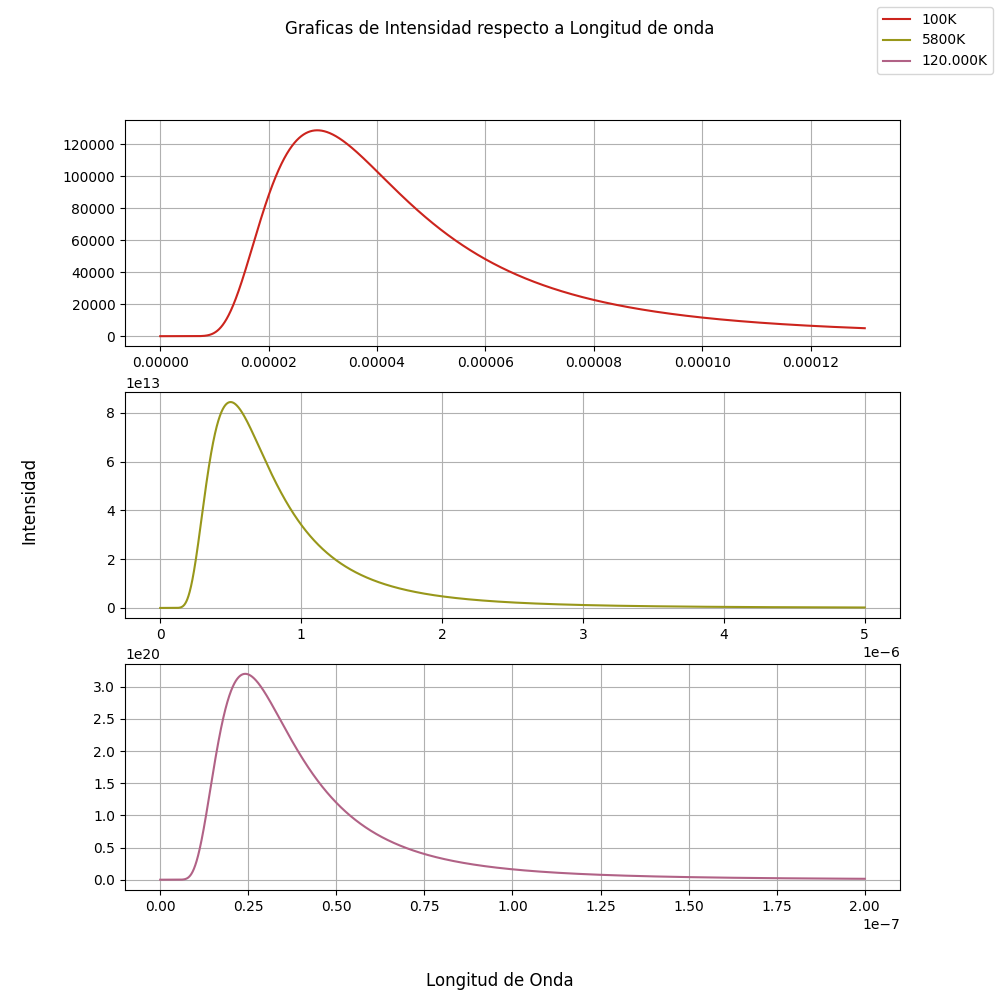
\includegraphics[width=0.8\textwidth]{img/General.png}
  \caption{Gráfica de Intensidad respecto a la longitud de onda}
  \label{fig:lng}
\end{figure}



\end{document}
